\documentclass[sigconf]{acmart}
% if you need to pass options to natbib, use, e.g.:
 \PassOptionsToPackage{numbers, compress}{natbib}
% before loading nips_2017
%
% to avoid loading the natbib package, add option nonatbib:
% \usepackage[nonatbib]{nips_2017}


\usepackage[utf8]{inputenc} % allow utf-8 input
\usepackage[T1]{fontenc}    % use 8-bit T1 fonts
\usepackage{hyperref}       % hyperlinks
\usepackage{url}            % simple URL typesetting
\usepackage{booktabs}       % professional-quality tables
\usepackage{amsfonts}       % blackboard math symbols
\usepackage{nicefrac}       % compact symbols for 1/2, etc.
\usepackage{microtype}      % microtypography
\usepackage{amsmath}
% Choose a title for your submission

\setcopyright{none}
\settopmatter{printacmref=false,printfolios=false}

\begin{document}

\title{3D Human Pose Estimation}


\author{Mounir Amrani}\affiliation{}
\email{mamrani@student.ethz.ch}
\author{Srikanth Gurram}\affiliation{}
\email{sgurram@student.ethz.ch}

\begin{abstract}
3D human pose estimation involves estimating human joint locations in 3D directly from 2D camera images. The estimation model would have to estimate the depth information directly from the 2D images. We explore two method in this paper both of which represent human pose as a heatmap. The first one follows (Newell et al. \cite{newell}) and (Martinez et al. \cite{martinez}) where we predict 2D poses and then lift these 2D poses to 3D. The second approach is inspired by (Pavlakos et al. \cite{pavlakos}) and involves learning 3D pose directly from the 2D images. We observe that while both these approaches work well, the mean of both their predictions gives us the best mean per-joint prediction error (MPJPE) score.
\end{abstract}

\maketitle

\section{Introduction}
\quad 3D Human Pose Estimation is a challenging task that generated a lot of attention for many years. Since most depictions of humans are 2D e.g. images, videos etc., many systems have been designed to estimate from these 2D images the 3D skeleton of the depicted person. Many applications would benefit from accurate 3D human pose estimation for e.g. virtual reality, augmented reality and autonomous driving. Perhaps the most challenging part of this problem is to infer the depth information given only a 2D image. Other challenges include handling occlusions and the different camera views. The system must also be invariant to changes in background, lighting, clothing etc.

With the recent successes of deep learning models in many computer vision tasks, research has been focused lately on developing a deep learning model to solve the 3D pose estimation task. There are 2 main approaches to this task: detection based approaches \cite{pavlakos} where the model generates a likelihood heatmap around each joint and locates the joint as the point with maximum likelihood and regression based approaches \cite{li} where the model directly estimates the 3D joint coordinates without generating an intermediate heatmap representation. Some recent work have successfully unified both approches \cite{sun}. Although detection based approaches perform quite well compared to regression based approaches, they suffer from quantization errors. We use the MPJPE as evaluation metric for both models. To help reduce the quantization error of the 2nd model, we combine the predictions of our 2 models by a simple per coordinate averaging operation and observe an important decrease in the MPJPE.

In this paper, we present 2 models: the first one combines detection of 2D joint coordinates by generating a 2D heatmap and a simple regression to lift those 2D coordinates to 3D, whereas the second one is purely detection based and generates a 3D heatmap for each joint.

We closely follow the implementations of \cite{newell}$^1$\footnote{$^1$https://github.com/princeton-vl/pose-hg-train}, \cite{martinez}$^2$\footnote{$^2$https://github.com/una-dinosauria/3d-pose-baseline} and \cite{pavlakos}$^3$\footnote{$^3$https://github.com/geopavlakos/c2f-vol-train/}.

We take the Tensorflow implementation of \cite{martinez} and modify it for our own purposes.

\section{Model}
\quad In the following, we describe the main component of our 2D and 3D detection approaches: the stacked hourglass architecture. This architecture has been proposed by \cite{newell} for 2D pose estimation and extended by \cite{pavlakos} for an end-to-end 3D pose estimation.

\begin{figure}
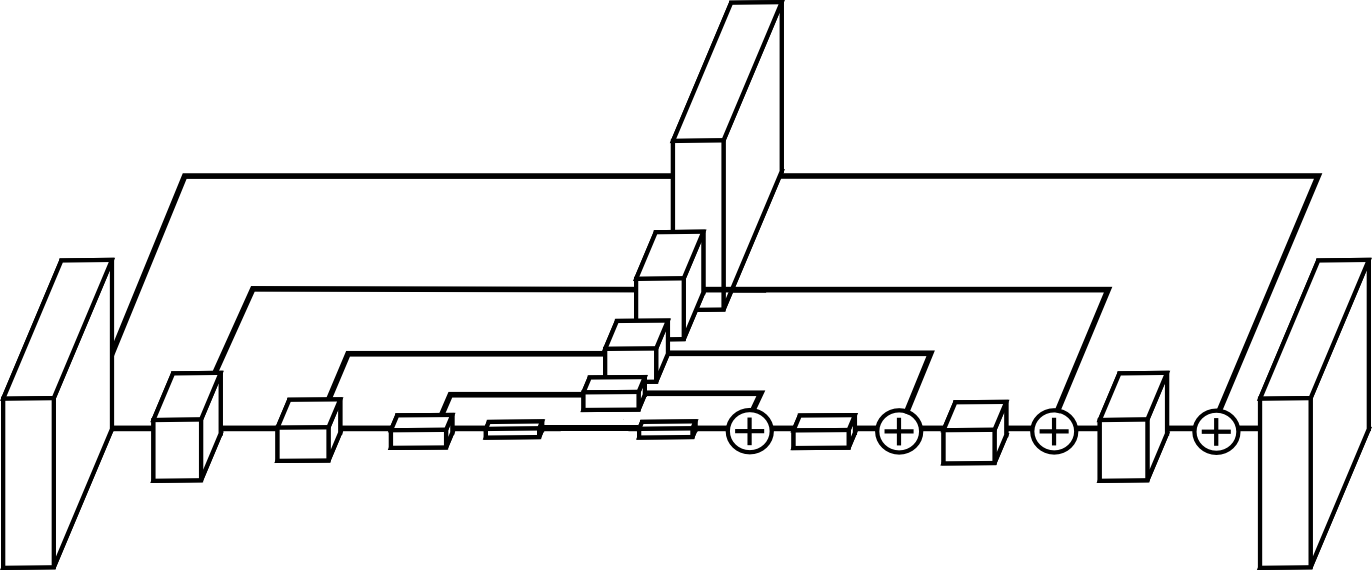
\includegraphics[height=1in, width=2.5in]{img/single-hourglass.png}
\caption{Hourglass module architecture from \cite{newell}}
\end{figure}

\subsection{The hourglass design}
\quad The main component of the stacked hourglass architecture is the hourglass (HG) module that can be seen in Figure 1. The input to the HG module has height H, width W and channels C. Both the input and output to the HG module have the same dimensions H, W and C, but H and W are modified inside the HG while C is preserved (here H=64, W=64 and C=256).

Each box is a called a "residual block" and contains $n$ successive "residual modules" (for us $n=1$). Each residual module is a succession of 3 "convolution blocks" and has a residual connection. Each convolution block is a succession of a batch normalization layer, a ReLU layer and a convolution layer. For each convolution block, the input's width and height are preserved and only the number of output channels changes.

The 1st convolution block has a 1x1 kernel, 1x1 stride, no padding and outputs C/2 channels. The 2nd convolution block has a 3x3 kernel, 1x1 stride, 1x1 padding and outputs C/2 channels. The 3rd convolution block has a 1x1 kernel, a 1x1 stride, no padding and outputs C channels.

Consider the left half of the HG module: before each residual block in the lower branch, there is a 2x2 max pooling layer with stride 2x2 to half the height and width of the input to the residual block. Only the last residual block isn't preceded by a max pooling layer (the smallest resolution HxW is 4x4). The input to the upper branch residual block is the input to the max pooling layer preceding the "corresponding lower branch residual block".

Consider the right half of the HG module: the output of each residual block in the lower branch is up-sampled with nearest neighbor up-sampling before summing it up with the output of the corresponding residual block of the upper branch. This is true for all residual blocks of the lower branch except the last one which is not followed by an up-sampling step.

One last linear block is applied to the output of the HG module. A Linear block is simply a convolution layer followed by a batch normalization layer followed by a ReLU layer. To get the HG module's 17 2D heatmaps predictions (1 per joint), a convolution layer with 17 output channels is applied on the linear block's output. Further, a convolution layer (conv1) with C output channels is applied after the linear block and a convolution layer with C output channels (conv2) is applied on the HG's heatmaps.

Finally, the HG module's input is summed up with the outputs of conv1 and conv2 to get the final output. Let us call this pipeline starting at the HG module's input and ending at the final output an "Hourglass block" (see Figure 2). All convolution layers that follow the HG module of the HG block have a with 1x1 kernel, 1x1 stride and no padding. 

\begin{figure}
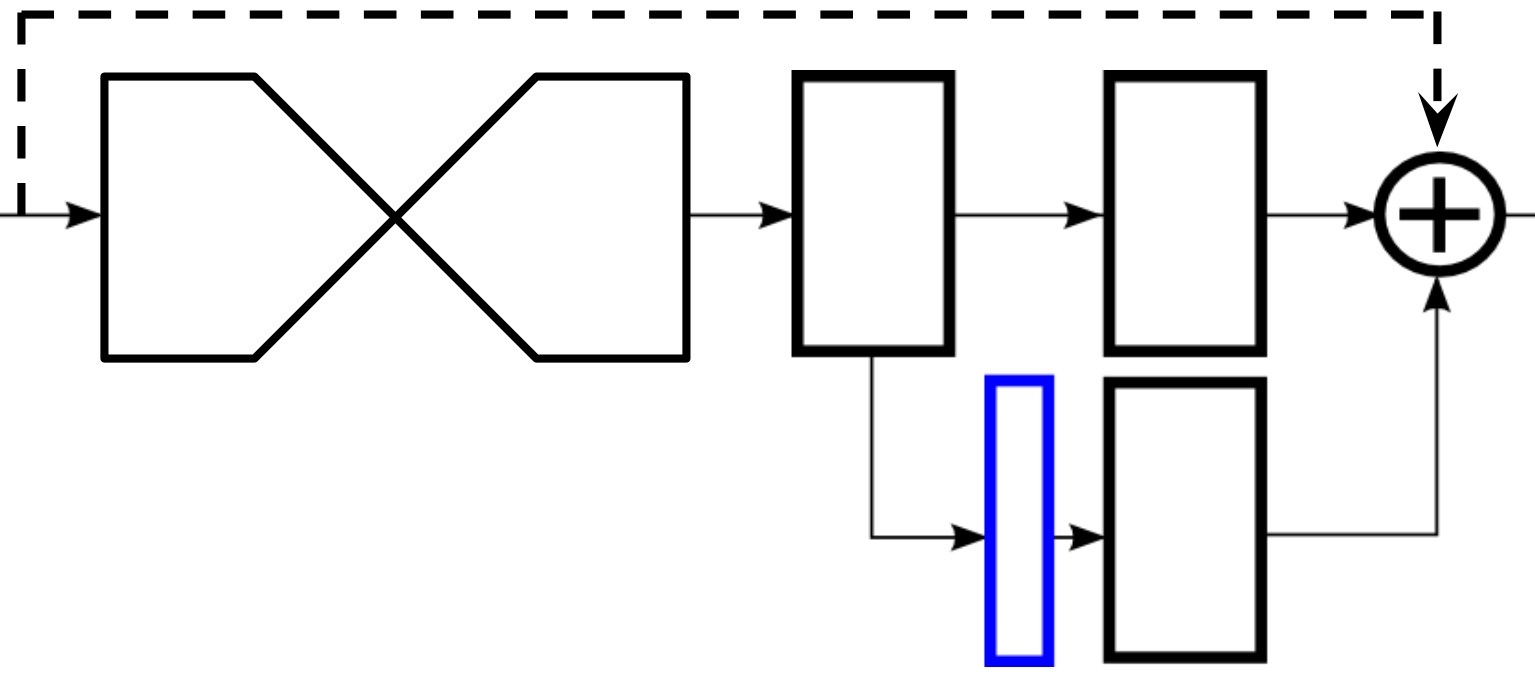
\includegraphics[height=0.7in, width=1.8in]{img/hg_block.png}
\caption{Hourglass block from \cite{newell}}
\end{figure}

\subsection{Stacked Hourglass}
\quad The stacked hourglass architecture is simply a succession of HG blocks (i,e we stack multiple HG blocks). This design choice allows for intermediate supervision where we apply a loss on the output heatmaps of each HG block. The loss used is simply the mean squared error (MSE) between the predicted heatmaps and the groud-truth heatmaps. The ground-truth heatmap of a joint is simply an unnormalized 2D Gaussian centered at the pixel position of the joint with standard deviation $\sigma$ (here $\sigma=1$)

Note here that in order to decrease the size of the model and thus its memory requirements, the input images of height 256 and width 256 are first preprocessed to get an input to the 1st HG block of resolution HxW=64x64 and C=256 channels. This means that the predicted heatmaps also have HxW=64x64. The predicted joint location is simply the pixel position of max value in the final output heatmap. These joint locations are scaled up to match the input image resolution which is 256x256.

We experiment with stacking 8 HG blocks and 4 HG blocks.
\subsection{Hourglass for 3D heatmaps}
\quad So far, the predicted heatmaps have only 2 dimensions both with resolution 64. In order to predict the 3rd dimension with resolution $z_i$ for the i'th HG block, we simply modify the i'th HG block to output 17*$z_i$ channels instead of 17 channels (so we get $z_i$ channels per joint)

We follow the coarse-to-fine approach described in \cite{pavlakos} where the resolution $z_i$ is increased from HG block to another until a final output resolution $z_{out}$ of the last HG block is reached (we choose $z_{out}=64$ to match the $x$ and $y$ resolution of the output).

The loss we apply is the summed square error (SSE) between the ground-truth 3D heatmaps and the predicted 3D heatmaps (SSE is like the MSE but instead of averaging, we sum), we also experiment with the MSE as loss.

The final output 3D heatmap is a (discretized) cube of voxels of resolution 64x64x64 and represents the metric space (x, y, z) $\in$ [-1000,1000] x [-1000, 1000] x [-1000, 1000] in mm where the root joint is always at (0, 0, 0) and the other joint's coordinates given w.r.t the root joint. In order to avoid dealing with negative values, we shift the ground-truth joints by 1000 mm in each axis so the root would be at (x, y, z) = (1000, 1000, 1000). So we have 64 units in voxel space correspond to 2000 units in metric space, for each axis. This gives a direct way to convert joint coordinates back and forth between voxel and metric space.

After converting each joint coordinates to voxel space, we generate an unnormalized 3D gaussian centered at the joint's voxel coordinates with $\sigma=2$ in each axis. This gives the 3D gaussian to be predicted by the last HG block. But since the z-resolution of 3D heatmap changes across the HG blocks, we also scale the variance along the z-axis of the 3D ground-truth gaussian to be predicted by the i'th HG block by a factor of $\frac{z_i}{z_{out}}$ for all i

Finally, the voxel coordinates with maximum value in the final output 3D heatmaps is chosen to be the location of the corresponding joint.

We operate the same changes to the architecture as \cite{pavlakos}$^1$\footnote{$^1$https://github.com/geopavlakos/c2f-vol-train/}. The main changes are in the number of channels preserved throughout the stacked HG blocks which becomes 512 and also few changes in the part of the HG block that follows the HG module.

We experiment with stacking 4 3D HG blocks with the following output z-resolutions: 1, 2, 4, 64.
\subsection{Lifting 2D pose to 3D}
We follow the exact same approach described in \cite{martinez} with the same architecture and same parameters. The network is a simple feed-forward neural network (FFNN) with batch normalization, dropout and relu activation as shown in Figure \ref{sb_arch}. The  2d pose is first lifted to $1024$ dimensions using a linear transformation followed by batch normalization, relu and dropout with dropout rate 0.5. This transformed 2d pose undergoes transformations as shown in Figure \ref{sb_arch} (note the use of 2 successive blocks of transformation). The resulting vector of $1024$ dimensions is projected down to $17*3$ dimensions using a simple linear transformation.

\begin{figure}
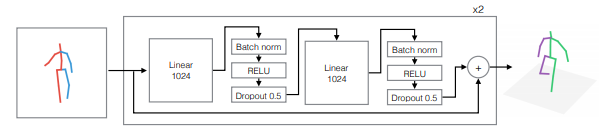
\includegraphics[height=0.75
in, width=3in]{img/sb_arch.png}
\caption{Network architecture to lift 2D pose to 3D pose described in \cite{martinez}}
\label{sb_arch}
\end{figure}

\section{Data}
\quad The dataset provided was a subset of the Human3.6M dataset with 312188 labeled images of size 256x256x3 and a test set of 10987 unlabeled images on which to perform predictions. The labels provided are the 2D pixel positions of the joints and 3D joint positions in mm w.r.t the root joint (pelvis) which is always at (0, 0, 0).

The labeled data contained images of subjects S1, S5, S6, S7 and S8, the unlabeled data contained subjects S9 and S11. During training, we experiment with data augmentation where each image is randomly rotated by a random angle in the range $[-30, 30]$ degrees.

\section{Training}
\quad For both the 2D and 3D hourglass models: We hold out 2188 for validation to estimate the validation loss and MPJPE and train on the 310k samples left. The data is shuffled and batched with batch size 4. Given the large size of the 3D hourglass network and increased dimensionality due to estimating the depth information, which made predictions rather slow, we only estimate the validation loss and accuracy as the mean over 10 batches. We initialize our model weights with xavier initialization. We train our model with Adam Optimizer and learning rate 2.5e-4, we also experiment with a learning rate of 0.001 on the 2D HG model, and experiment with learning rate decay (where we half the learning rate every epoch) for both 2D and 3D HG models. We train each model for 4 epochs and predict pose estimates for test data after every epoch.

For the feed-forward approach: We use all the labeled data to perform training. The 2D and 3D poses are normalized by using a standard scaler that performs mean correction and scales the data to have unit variance. The model parameters are initialized using kaiming initialization as described in \cite{kaim}. Since this model is fairly light, we train this model for 200 epochs with a batch size of 64. We update the model parameters using Adam optimizer with a learning rate of $0.001$. We decay the learning rate after every $100000$ steps using an exponential decay with an exponent of $0.96$. Since the model is fairly simple, we use the training data without performing any augmentation.

\section{Experiments results}
We present in the following the results from our different experiments, these are the MPJPE scores achieved by our predictions on the public split of the submission system: 

For 2D HG model + FFNN: Our best result was 109.02 and were achieved by the use of 8 stacked HG blocks with data augmentation and a fixed learning rate of 2.5e-4 after 2 epochs of training. A close result of 110.34 was achieved by the use of 4 stacked HG blocks with data augmentation and a decaying learning rate starting at 0.001. The best result achieved without data augmentation was 112.16 by training for 1 epoch with fixed learning rate of 0.001.

For the 3D HG model: Our best result was 99.17 achieved by training for 4 epochs with SSE loss, no data augmentation and a fixed learning rate of 2.5e-4. The closest result achieved by using MSE loss was 102.17 by training for 4 epochs with no data augmentation and fixed learning rate of 2.5e-4. Although the 2D HG model seemed to benefit from the data augmentation and learning rate decay, the 3D HG model seemed to suffer from both of them since adding them gave us a best result of 118.28 after 4 epochs and leaning rate starting at 2.5e-4.

Our best score was 89.69 and achieved by taking a per-coordinate average of the predictions with best score for each of the above models. This allows to lower the effect of quantization errors of the 3D HG model and thus give better predictions.

\section{Qualitative results}
\quad Figure 4 and Figure 5 show 2 samples images of the test set and our best predictions on each image with 2 view points. As can be seen in Figure 4, the pose estimated is qualitatively similar to the pose of the person depicted in the image, whereas Figure 5 shows a failure case of our model: we assume that this is due to the training set having few poses as in this image since most images in the pose depict a person is a Standing or Sitting position, also this image contains many occlusions like occlusion of the head which may have made it harder for our model to accurately predict the pose.

\begin{figure}
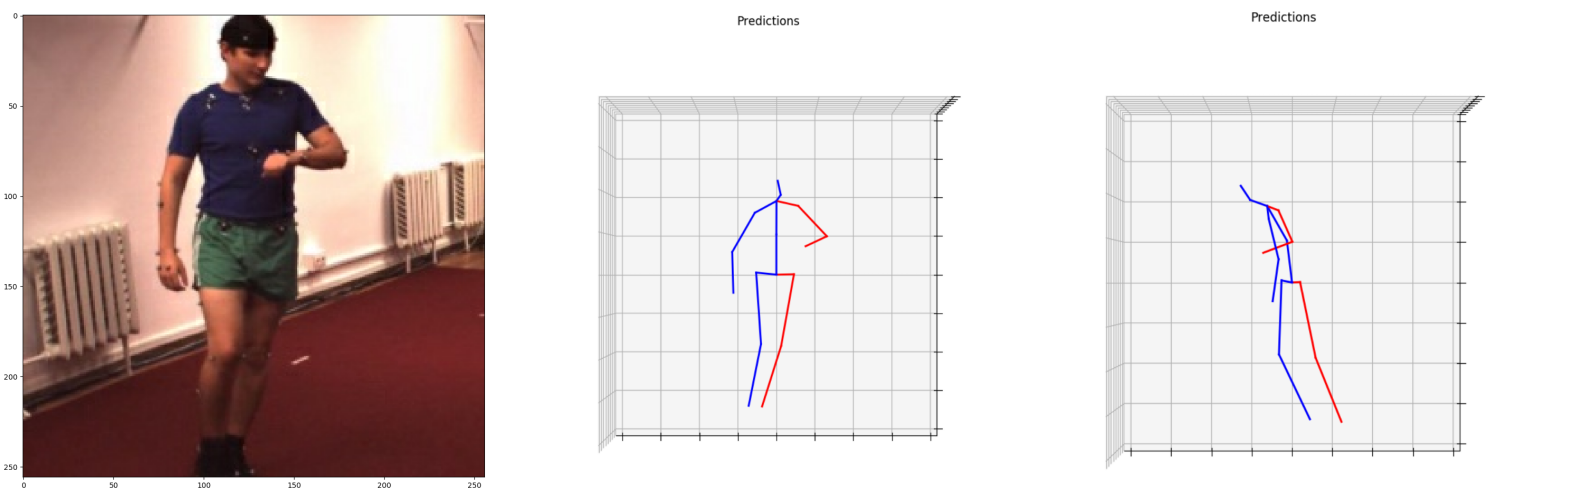
\includegraphics[height=1in, width=2.5in]{img/success.png}
\caption{A success case of our best predictions}
\end{figure}

\begin{figure}
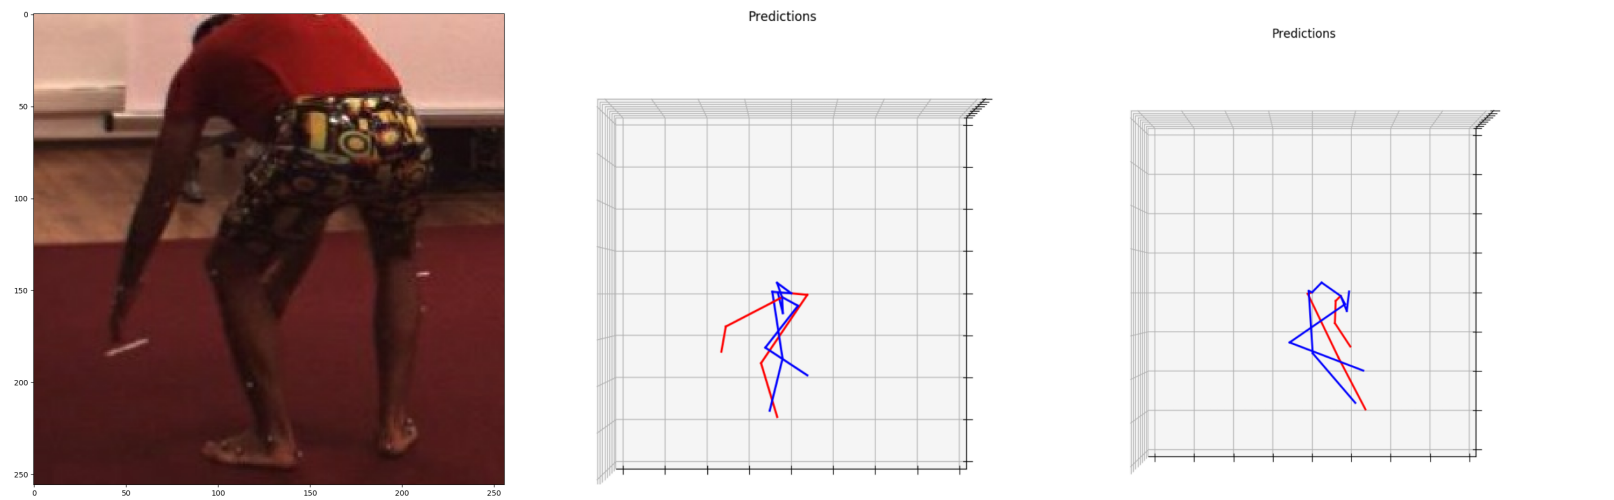
\includegraphics[height=1in, width=2.5in]{img/failure.png}
\caption{A failure case of our best predictions}
\end{figure}

\section{Conclusion}
\quad We show the effectiveness of hourglass based models in estimating 3d pose from 2D images. Both the approaches discussed here rely on stacked hourglass models to estimate 2D/3D poses directly from images. We develop a simple and effective way of training these models and achieve a mean per-joint prediction error (MPJPE) score of 89.69 mm using a combination of both the 3D hourglass model and the 2D hourglass + FFNN. 
\begin{thebibliography}{}
 
\bibitem{newell} A. Newell, K. Yang, and J. Deng (2016): Stacked Hourglass Networks for Human Pose Estimation

\bibitem{martinez} J. Martinez, R. Hossain, J. Romero and J. J. Little (2017): A simple yet effective baseline for 3d human pose estimation

\bibitem{pavlakos} G. Pavlakos, X. Zhou, K. G. Derpanis, K. Daniilidis (2017): Coarse-to-Fine Volumetric Prediction for Single-Image 3D Human Pose

\bibitem{li} S. Li and A. B. Chan (2014): 3D human pose estimation from
monocular images with deep convolutional neural network.

\bibitem{sun} X. Sun, B. Xiao, F. Wei, S. Liang, and Y. Wei (2018): Integral Human Pose Regression

\bibitem{kaim} Kaiming He, Xiangyu Zhang, Shaoqing Ren, Jian Sun (2015): Delving Deep into Rectifiers: Surpassing Human-Level Performance on ImageNet Classification

\end{thebibliography}
\newpage
\end{document}